\cotefile{130}
\scanpage{20}
% archive sheet number: 10 (inverted)
\mspage{-VII- 9 -}\hfill n°383

4. \uline{Schémas de Dynkin}.

Soient $S$ un système de racines réduit, $G$ son groupe de Weyl, $(u_1,\ldots,u_r)$ ses racines simples relatives à une chambre. Posons $n(i,j)=2(u_i\mid u_j)/(u_i\mid u_i)$. D'après le \S~4, n°2, les seuls cas possibles, pour $i\ne j$, sont les suivants (en tenant compte du fait que l'angle de deux racines simples est obtus ; cf.\ \S~3, n°1, prop.2) :

\[
\begin{aligned}
1)\ & n(i,j)=n(\unsure{j|J},i)=0\ ;\ (u_i,u_j)=\handwritten{\pi}/2\ ;\ s_i s_j=-1\\
2)\ & n(i,j)=n(j,i)=-1\ ;\ (u_i,u_j)=2\handwritten{\pi}/3\ ;\ s_i s_j\ \text{d'ordre }3\ ;\ \|u_i\|=\|u_j\|\\
3)\ & n(i,j)=-1,\ n(j,i)=-2\ ;\ (u_i,u_j)=3\handwritten{\pi}/4\ ;\ s_i s_j\ \text{d'ordre }4\ ;\ \|u_i\|=\handwritten{\sqrt{2}}\,\|u_j\|
\end{aligned}
\]
(ou ce qu'on obtient en échangeant $i$ et $j$)
\[
4)\quad n(i,j)=-1,\ n(j,i)=-3\ ;\ (u_i,u_j)=5\handwritten{\pi}/6\ ;\ s_i s_j\ \text{d'ordre }6\ ;\ \|u_i\|=\handwritten{\sqrt{3}}\,\|u_j\|
\]
(ou ce qu'on obtient en échangeant $i$ et $j$).

Nous appellerons \uline{schéma de Dynkin} de $S$ le graphe à $r$ noeuds $1,2,\ldots,r$ dont les simplexes sont les parties $\handwritten{\{}i,j\handwritten{\}}$ à deux éléments telles que $(u_i\mid u_j)\ne0$, chaque noeud $i$ étant affecté du coefficient $\|u_i\|^2$. Le graphe sous-jacent à ce schéma n'est autre que le graphe de $G$. Les remarques précédentes permettent de reconstituer le schéma de Coxeter de $G$ à partir du schéma de Dynkin de $S$ (mais pas inversement).

PROPOSITION 2.- \uline{Soient} $V,V'$ \uline{des espaces hilbertiens réels de dimension finie}, $S$ (resp.\ $S'$) \uline{un système de racines réduit dans} $V$ (resp.\ $V'$), $u_1,\ldots,u_r$ (resp.\ $u'_1,\ldots,u'_{r'}$) \uline{les racines simples de} $S$ (resp.$S'$) \uline{relatives à une chambre}. \uline{S'il existe un isomorphisme} $i\handwritten{\rightsquigarrow}j(i)$ \uline{du schéma de Dynkin de} $S$ \uline{sur celui de} $S'$, \uline{il existe un isomorphisme de} $V$ \uline{sur} $V'$ \uline{transformant} $u_i$ \uline{en} $u'_{j(i)}$ \uline{pour tout} $i$, \uline{et} $S$ \uline{en} $S'$.

En effet les hypothèses et les remarques ci-dessus entraînent que $r=r'$ et que $(u_i\mid u_k)=(u'_{j(i)}\mid u'_{j(k)})$ quels que soient $i$ et $k$. Donc l'application $x_1u_1+\ldots+x_ru_r\handwritten{\rightsquigarrow}x_1u'_{j(1)}+\ldots+x_ru'_{j(r)}$ est un isomorphisme $f$ de $V$ sur $V'$, qui transforme le groupe de Weyl $G$ de $S$ en le groupe de Weyl $G'$ de $S'$. Or $S$ (resp.\ $S'$)

\scanpage{22}
% archive sheet number: 21
\diagram{\begin{tikzcd}[ampersand replacement=\&]
X \arrow[d,"f"]\\ S
\end{tikzcd}}
\[
\begin{aligned}
-\langle D_{\eta},C_{\eta}\rangle&=D.C\\[-2pt]
\rotatebox{90}{$=$}&\\[-2pt]
\sum_v\langle D_{\eta},C_{\eta}\rangle_v&=\sum_v(D.C)_v
\end{aligned}
\]
\margin{si $D_{\eta}$ et $C_{\eta}$ alg. équiv. à $0$}

$f$ projectif : fibres \inserted{géom.} \uline{irréductibles}, \uline{fibre générique lisse}, $X$ régulier ; $S$ muni d'un \unsure{ens.|ensemble} $M$ de val. abs. discrètes satisfaisant la formule du produit

\smallskip\hrule\smallskip

$S$ local complet corps résiduel alg. clos

$X\leftarrow S$ projectif, $X_{\eta}$ lisse,

$X_0$ lisse sauf \unsure{au} plus en un pt, \unsure{ou|on|ces} \unsure{disons|derniers} étant en plus $X$ \uline{régulier} \inserted{\unsure{p. ex. disons|pr. indiqué|en ces pts}}.

$C,D$ sur $X$,
\[
\left.
\begin{array}{l}
\deleted{\text{se}}\quad
\left\{\begin{array}{l}
\deleted{\text{\unsure{prop.}}}\ \text{\inserted{sans} comp. verticales}\\
\deleted{C.D}\ \operatorname{supp} C\cap\operatorname{supp} D\subset X_0
\end{array}\right.
\end{array}
\right\}=\text{\unsure{Se|Ils} \unsure{coupant|coupent} avec la bonne dimension}
\]

$C_{\eta},D_{\eta}$ alg. équiv. à $0$ sur $X_{\eta}$

\[
\boxed{\langle C_{\eta},D_{\eta}\rangle_v=i(C.D)}
\]
\margin{\deleted{\unsure{exceptons} sauf \unsure{en} \unsure{$g$}}}

\scanpage{23}
% archive sheet number: 22
\mspage{-II- 13 -}
l'adhérence d'une face de $g'(C)$. De plus, si $h(W_i)=g'(W_k)$, on a $r_p h(W_i)=r_p g'(W_k)$, d'où, par $(\mathrm{II}_{m-1})$, $(r_p h)r_i(r_p h)^{-1}=(r_p g')r_k(r_p g')^{-1}$ ; ceci donne aussitôt $hr_i h^{-1}=g'r_k g'^{-1}$. On a donc démontré $(\mathrm{II}_m)$ dans le second cas.

LEMME 5.- \uline{Soit} $g=r_{i_1}\ldots r_{i_m}\in G$, \uline{et soit} $W_j$ \uline{un mur}. \uline{Si les chambres} $C$ \uline{et} $g(C)$ \uline{sont de part et d'autre de} $W_j$, \uline{alors} $r_j g$ \uline{est un produit de} $m-1$ \uline{générateurs} $r_{i_k}$.

Considérons, en effet, la suite de chambres $C_k=r_{i_1}\ldots r_{i_k}(C)$ $(k=0,\ldots,m)$ ; on a $C_{\unsure{o|0}}=C$ et $C_m=g(C)$. Il existe deux éléments consécutifs de cette suite qui sont de part et d'autre de $W_j$, soient $C_{q-1}$ et $C_q$. Posons $h=r_{i_1}\ldots r_{i_{q-1}}$, de sorte que $C_{q-1}=h(C)$ et $C_q=hr_{i_q}(C)$. Comme $C$ et $r_{i_q}(C)$ ont en commun la face $W_{i_q}\cap\overline C$ de dimension $n-1$, $C_{q-1}$ et $C_q$ ont en commun une face $F$ de dimension $n-1$ contenue dans $h(W_{i_q})$. On a $F\subset\overline C_q\cap\overline C_{q-1}$, d'où $F\subset W_j$ puisque $C_{q-1}$ et $C_q$ sont de part et d'autre de $W_j$ ; comme $F$ engendre l'hyperplan $h(W_{i_q})$, on a donc $W_j\supset h(W_{i_q})$ et $W_j=h(W_{i_q})$ (puisqu'il s'agit de deux \unsure{hyperplans|hyperplens}). Le lemme 4 montre qu'on a $r_j=hr_{i_q}h^{-1}$, d'où
\[
r_jg=r_jhr_{i_q}r_{i_{q+1}}\ldots r_{i_m}
=hr_{i_q}r_{i_q}r_{i_{q+1}}\ldots r_{i_m}
=r_{i_1}\ldots r_{i_{q-1}}r_{i_{q+1}}\ldots r_{i_m},
\]
ce qui démontre notre assertion.

LEMME 6.- \uline{Soit} $g\in G$. \uline{Si} $g(C)\cap C\ne\varnothing$, \uline{alors} $g=1$.

En vertu du lemme 3, $g(C)$ ne rencontre aucun $W_i$ ; donc, si $g(C)\cap C\ne\varnothing$, on a $g(C)\subset C$ puisque $g(C)$ est connexe ; de même on a $g^{-1}(C)\subset C$, d'où $C\subset g(C)$ et $C=g(C)$. Supposons $g\ne1$, et exprimons-le comme un produit $g=r_{i_1}\ldots r_{i_m}$ de longueur minimum. Les chambres $C$ et $r_{i_1}(C)=r_{i_2}\ldots r_{i_m}(C)$ sont situées de part et d'autre de $W_{i_1}$ ; donc, d'après le lemme 5, $r_{i_1}(r_{i_2}\ldots r_{i_m})=g$ peut s'écrire sous la forme d'un

\scanpage{24}
% archive sheet number: 23
$A$ anneau local \inserted{\unsure{noeth|noeth.}} réduit de dim $2$,

de profondeur $\deleted{\unsure{=}}2$

$f\in\unsure{\mathfrak r|\mathfrak m}A$ tel que $A/fA$ est régulier

\noindent\begin{tikzpicture}[x=\linewidth,y=1em]
\draw (0,0) -- (.91,0); \draw (.82,1.6) -- (.82,-.8);
\end{tikzpicture}

\diagram{\begin{tikzcd}[ampersand replacement=\&,column sep=small,row sep=small]
\& X \arrow[dl] \arrow[d,dash] \& A\supset B\\
{} \& {} \& B\times B'
\end{tikzcd}}
\diagram{\begin{tikzcd}[ampersand replacement=\&,row sep=small]
B_{\eta} \& A_{\eta}\arrow[l,"\beta"'] \& B_{\eta}\arrow[l,"\alpha"']\arrow[ll,bend right=28,"N"']\\
B \& A\arrow[l]\arrow[u] \& B\arrow[l]
\end{tikzcd}}

$A_{\eta}=A_{1\eta}\times A_{2\eta}$ \quad $A$ OK.

\[
\begin{aligned}
B_1&=\overline{A_{1\eta}} \quad A \qquad X \qquad N_{\eta} \qquad A\unsure{\subset|\leftarrow}B\\
B_2&=\overline{A_{2\eta}}
\end{aligned}
\]

\diagram{\begin{tikzcd}[ampersand replacement=\&,row sep=small]
A \& \unsure{\text{---}|\rightarrow} \& \overline{A_{1\eta}}\\
A\arrow[rr] \& {} \& \overline{A_{2\eta}}
\end{tikzcd}}
\diagram{\begin{tikzcd}[ampersand replacement=\&,row sep=small]
\& A\arrow[r,shift right] \& \deleted{\unsure{A}}B_1\times B_2\arrow[l,shift right]\\
\deleted{B_1\times B_2}\arrow[ur] \& \&
\end{tikzcd}}

\diagram{\begin{tikzcd}[ampersand replacement=\&,row sep=small,column sep=small]
0\arrow[d] \& 0\arrow[d,dash] \& \overline A\\
A\arrow[u,shift left] \& \check A\arrow[d] \& {}\\
B\arrow[u] \& \unsure{\check B|\check D}\arrow[d] \& B\arrow[d]\\
C\arrow[u] \& \check C \& C
\end{tikzcd}}

\diagram{\begin{tikzcd}[ampersand replacement=\&,row sep=small]
\& T\arrow[dl]\\
A_{\unsure{.|\circ}}\&\deleted{B}\\
A_{\eta}\& B_{\eta}\arrow[l]\\
\&T_{\eta}\arrow[u]
\end{tikzcd}}

\figure{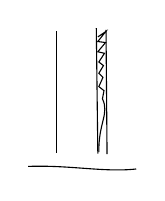
\begin{tikzpicture}[x=.65cm,y=.65cm]
\draw (0,.22)--(0,2.6);
\draw (.8,.2)--(.77,2.65) (.98,.19)--(.96,2.62);
\draw (.82,.23) .. controls (.81,.8) and (1.03,.98) .. (.89,1.27)
 --(.92,1.43)--(.82,1.51)--(.9,1.69)--(.82,1.77)--(.91,1.92)--(.82,1.99)
 --(.93,2.16)--(.8,2.19)--(.95,2.37)--(.8,2.39)--(.95,2.58)--(.8,2.48);
\draw (-.56,-.05) .. controls (.26,-.02) and (.93,-.17) .. (1.55,-.1);
\end{tikzpicture}}

\diagram{\begin{tikzcd}[ampersand replacement=\&,row sep=small]
A\arrow[d,very thick]\\ S
\end{tikzcd}}

\scanpage{25}
% archive sheet number: 24 (inverted)
\mspage{-I- 1 -}\hfill \handwritten{n°383}

\S~1. \uuline{Résultats préliminaires}.

1. \uline{Lemmes sur les chambres}.

Soit $V$ un espace vectoriel réel de dimension finie.

DEFINITION 1.- \uline{Une partie} $C$ \uline{de} $V$ \uline{est appelée une chambre si elle est non-vide et s'il existe une famille localement finie} $\underline H$ (Top. Gén., I, \handwritten{3}ème éd., \S~1, n°\handwritten{5}, déf.8) \uline{d'hyperplans affines de} $V$ \uline{et}, \uline{pour tout} $H\in\underline H$, \uline{un demi-espace ouvert} $D_H(C)$ \uline{défini par} $H$ \uline{tels que} $C=\displaystyle\bigcap_{H\in\underline H}D_H(C)$.

Un point quelconque $x$ de $C$ n'est dans aucun hyperplan $H\in\underline H$ ; comme $\underline H$ est localement finie, il existe une boule de centre $x$ qui ne rencontre aucun $H\in\underline H$, et qui est donc contenue dans chaque demi\unsure{-|.}espace $D_H(C)$ ; il en résulte que toute chambre est \uline{ouverte}. Il est clair que toute chambre est \uline{convexe}.

DEFINITION 2.- \uline{Soit} $C$ \uline{une chambre}. \uline{Un hyperplan affine} $L$ \uline{de} $V$ \uline{est appelé un mur de} $C$ \uline{s'il existe un demi-espace ouvert} $L^+$ \uline{défini par} $L$, \uline{un point} $x$ \uline{de} $L$ \uline{et un voisinage} $U$ \uline{de} $x$ \uline{tels que} $U\cap L^+=U\cap C$.

LEMME 1.- \uline{Soient} $L,L'$ \uline{deux hyperplans affines de} $V$, $L^+$ \uline{et} $L^-$ (resp.\ $L^{\prime+}$ \uline{et} $L^{\prime-}$) \uline{les demi-espaces ouverts définis par} $L$ (resp.\ $L'$). \uline{S'il existe un point} $x$ \uline{de} $L\cap L'$ \uline{et un voisinage} $U$ \uline{de} $x$ \uline{tels que} $U\cap L^+\subset L^{\prime+}$, \uline{alors} $L^+=L^{\prime+}$, $L^-=L^{\prime-}$ \uline{et} $L=L'$.

Par translation on se ramène au cas où $x=0$. Comme tout élément de $L^+$ se déduit \margin{\handwritten{\unsure{$>$}}} d'un élément de $U\cap L^+$ par une homothétie de rapport $>0$, on a $L^+\subset L^{\prime+}$ ; d'où, par symétrie, $L^-\subset L^{\prime-}$, et donc $L^+\cup L^-\subset L^{\prime+}\cap L^{\prime-}$. Par passage aux complémentaires on en déduit $L'\subset L$, d'où $L'=L$ car ce sont des hyperplans. Par conséquent $L^+=L^{\prime+}$ et $L^-=L^{\prime-}$.

LEMME 2.- \uline{Soient} $C$ \uline{une chambre de} $V$, $\underline H$ \uline{une famille localement finie d'hyperplans telle que} $C=\displaystyle\bigcap_{H\in\underline H}D_H(C)$, \uline{et} $\underline H'$ \uline{la famille des murs de} $C$. \uline{Alors} :

\scanpage{26}
% archive sheet number: 25
\[
\begin{aligned}
\langle C_{\eta},\operatorname{div} f_{\eta}\rangle_v
  &=i(C.\deleted{\overline{\operatorname{div} f_{\eta}}})\\
\rotatebox{90}{$=$}&\\
\unsure{=|\Leftrightarrow}\ v(f_{\eta}(C_{\eta}))&
\end{aligned}
\]
\diagram{\begin{tikzcd}[ampersand replacement=\&,column sep=small]
X'\arrow[r,hook,"\text{\unsure{imm. ouverte}}"] \& \widetilde X''\arrow[r,"\text{\uline{fini} \uline{\unsure{birat|birat.}}}"] \& X'' \arrow[r,phantom,"\overset{\text{\unsure{imm. fermée}}}{\subset}"] \& J
\end{tikzcd}}

\diagram{\begin{tikzcd}[ampersand replacement=\&,row sep=small]
X'\arrow[r,hook]\arrow[d,dash] \& J\\
S\&\\[-3pt]\&S
\end{tikzcd}}
\figure{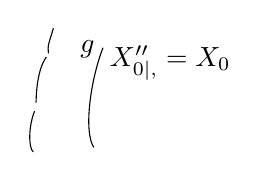
\begin{tikzpicture}[x=.45cm,y=.45cm]
\draw (0,2.8) .. controls (-.1,2.45) and (-.18,2.3) .. (-.14,2.09);
\draw (-.2,1.99) .. controls (-.43,1.65) and (-.48,1.12) .. (-.49,.7);
\draw (-.53,.46) .. controls (-.7,.05) and (-.71,-.57) .. (-.57,-.69);
\draw (1.4,2.25) .. controls (1.04,1.32) and (.85,-.12) .. (1.14,-.56);
\node at (.96,2.2) {$\deleted{\unsure{g}}$};
\node[anchor=west] at (1.32,1.83) {$X''_{\unsure{0|,}}=X_0$};
\end{tikzpicture}}
\diagram{\begin{tikzcd}[ampersand replacement=\&,row sep=small]
\unsure{K_{\eta}|k_{\eta}|X_{\eta}} \& X\arrow[d,dash]\\
\eta \& S\ \text{\unsure{spec. ann.} de val. discrète}
\end{tikzcd}}

\noindent\rule{2cm}{.4pt}

$x\in X_{\eta}(k(\eta))$\quad $\exists\ L$ faisceau loc. libre sur $X$ et une section rationnelle dont \deleted{\unsure{le|la}} diviseur sur $X_{\eta}$ est \unsure{réduit} : $(x)$

En \unsure{normalisant|modifiant}, on peut supposer que cette section est définie partout \uline{sauf} \unsure{en|au} \deleted{$x\in X_{\unsure{.}}$} le pt critique $x_0$, et que \deleted{elle \unsure{est}} son diviseur n'a pas de composante verticale. \unsure{Cela|Ceci} \unsure{que|car} \unsure{pour|que} la section donnée est un diviseur

\figure{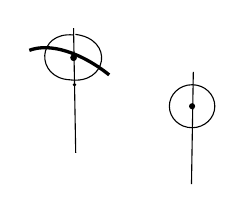
\begin{tikzpicture}[x=.78cm,y=.78cm]
\draw (0,1.58)--(.035,-.45);
\draw (0,1.47) .. controls (-.6,1.53) and (-.63,.77) .. (-.06,.74)
 .. controls (.55,.66) and (.67,1.4) .. (.03,1.48);
\draw[very thick] (-.72,1.22) .. controls (-.38,1.35) and (.13,1.18) .. (.58,.82);
\fill (0,1.10) circle (.055) (.015,.66) circle (.03);
\draw (1.95,.87)--(1.92,-.96);
\draw (1.93,.31) ellipse (.37 and .35);
\fill (1.93,.31) circle (.05);
\end{tikzpicture}}

\scanpage{27}
% archive sheet number: 26 (inverted)
\mspage{-I- 2 -}
a) \uline{on a} $\underline H'\subset\underline H$ ;

b) \uline{si} $H_{\unsure{o|0}}\in\underline H$ \uline{est tel que} $C'=\displaystyle\bigcap_{H\in\underline H,H\ne H_o}D_H(C)$ \uline{soit distincte de} $C$, \uline{alors} $H_o$ \uline{est un mur de} $C$ ;

c) \uline{on a} $C=\displaystyle\bigcap_{H\in\underline H'}D_H(C)$.

Soient $L\in\underline H'$ un mur de $H$, $x$ un point de $L$ et $U$ un voisinage de $x$ tels que $U\cap C=U\cap L^+$. Si $x$ n'appartenait \unsure{à|a} aucun $H\in\underline H$, il existerait une boule ouverte $B$ de centre $x$ telle que $B\cap H=\varnothing$ pour tout $H\in\underline H$ (car $\underline H$ est localement finie) ; on pourrait supposer que $B\subset U$, de sorte que $B\cap C=B\cap L^+$ ; comme $B\cap C$ est non-vide et que $B$ est connexe, on aurait $B\subset D_H(C)$, de sorte que $B\subset C$, d'où $x\in C$, en contradiction avec $x\in L^+$. Il existe donc $H\in\underline H$ tel que $x\in\underline H$ ; on a $U\cap L^+\subset C\cap D_H(C)$, d'où $H=L$ d'après le lemme 1. On a donc $\underline H'\subset\underline H$, ce qui démontre a).

Démontrons b). On a $C'\not\subset D_{H_o}(C)$. Comme $C'$ est convexe, on a donc $C'\cap H_o\ne\varnothing$ ; notons que $C'\cap H_o$ est relativement ouvert dans $H_o$. Les $H\cap H_o$, pour $H\in\underline H$ et $H\ne H_o$, forment une famille localement finie de sous-espaces affines de $H_o$ ; leur réunion est donc fermée et sans point intérieur, et ne peut par conséquent contenir $C'\cap H_o$. Il existe donc un point $y$ de $C'\cap H_o$ qui n'appartient à aucun $H\in\underline H$ distinct de $H_o$. Comme $\underline H$ est localement finie, il existe un voisinage ouvert convexe $U$ de $y$ tel que $U\cap H=\varnothing$ pour tout $H\in\underline H$, $H\ne H_o$. On a $U\cap C'\ne\varnothing$, d'où $U\cap D_H(C)\ne\varnothing$ pour tout $H\in\underline H$, $H\ne H_o$ ; comme $U$ est un ouvert convexe qui ne rencontre pas $H$, on en déduit $U\subset D_H(C)$. On a donc $U\cap C=U\cap(\displaystyle\bigcap_{H\ne H_o}D_H(C))\cap D_{H_o}(C)=U\cap D_{H_o}(C)$, de sorte que $H_o$ est un mur de $C$. Ceci démontre b).

Passons à c). Soit $z$ un point quelconque de $V$. Joignons-le à un point $y$ de $C$. Comme $\underline H$ est localement finie, le segment $[z,y]$ ne peut rencontrer qu'un nombre fini \margin{\handwritten{$\vert$}}d'hyperplans $H\in\underline H$. Donc les hyperplans $H\in\underline H$ tels que $z\notin D_H(C)$ sont en nombre fini, soient $H_1,\ldots,H_q$. Prenons alors pour $z$ un point de $\displaystyle\bigcap_{H\in\underline H'}D_H(C)$, de sorte que

\scanpage{28}
% archive sheet number: 27
$\unsure{*|a})$ Cas où $f$ est lisse, alors $X_{\eta}/\unsure{\xi|S|\eta|K}$ a un Albanese $A_{\eta}/\xi$ et $\operatorname{Picard}^{00}$ $A_{\eta}^{*}/\xi$, \deleted{\unsure{enfin}}, \inserted{\unsure{supp.} \unsure{à|a} une bonne réduction d'où $A,A^*$ ; \unsure{$\in$}} \inserted{\unsure{tenant compte} d'une section de $X$ sur $S$}, \deleted{un Albanese un \unsure{projectif}} et Th. de Weil, on a

\diagram{\begin{tikzcd}[ampersand replacement=\&]
X\arrow[rr,"\alpha"]\arrow[dr,dash] \& \& A\arrow[dl,dash]\\
\& S \&
\end{tikzcd}}

\deleted{et \unsure{on a}} \deleted{\unsure{et|de $X$} sur $A_{\eta}$ on a}

\deleted{$D_{\eta}'$ tel que $\alpha^*(D'_{\eta})\sim_{\unsure{\ell|l}}D_{\eta}$, d'où}

\[
\deleted{\alpha^*(D'_{\eta})=D_{\eta}+\operatorname{div}_{X_{\eta}}(f)}
\]
\deleted{d'où en prenant les adhérences}

\[
\deleted{D=\overline{D_{\eta}}=\alpha^*(\overline{D'_{\eta}}}
\]

Supposons d'abord que l'on ait
\[
D=\alpha^{\unsure{*|?}}\unsure{(|\,}D')
\]
$D'$ un diviseur sur $A$ sans \deleted{\unsure{comp. verticales}} tel que $\alpha^{*}(\unsure{D|D'})$ défini

Posons
\[
C'=\alpha_*(C)
\]
Alors on a
\[
C'.D'=\alpha_*(C).D'=\alpha_*(C\ \alpha^*(D'))=\alpha_*(C.D)
\]
d'où
\[
i(C.D)=i(\alpha_{\unsure{\alpha|*}}(C.D))\unsure{-|=}i(C'.D')
\]

\scanpage{29}
% archive sheet number: 28 (inverted)
\mspage{- e -}\hfill n°383

Le rédacteur n'a pas essayé, faute de compétence, de rédiger un laius expliquant où servent ces systèmes de racines ; le mieux qu'il aurait pu faire eût été de recopier Cartier (rédaction n°325), chose tout à fait inutile. D'ailleurs le laius de Cartier a été vomi, et le rédacteur n'aime pas du tout voir vider ce qu'il a rédigé.

Car il espère bien que c'est le dernier état, et qu'il sera envoyé in toto, illico, et maxima cum laude A L'IMPRESSION !!!!

\begin{center}\texttt{-:-:-:-}\end{center}

\scanpage{30}
% archive sheet number: 29
et notre formule dans ce cas se réduit à
\[
\boxed{i(\overline{C'_{\eta}},\overline{D'_{\eta}})=
 \langle C'_{\eta},D'_{\eta}\rangle_v}
\]
\margin{\deleted{si $C',D'$ sans \unsure{composantes}}}

Or \inserted{dans} le cas général, on \unsure{voit|sait} aussitôt qu'on aura
\[
D_{\eta}\sim\alpha^*(D'_{\eta}),
\]
où $D'_{\eta}$ est un diviseur sur $A_{\eta}$ tel que
\[
{\overset{\deleted{-}}{D'_{\eta}}}\not\supset\alpha_{\eta}(X_{\eta})
\quad\text{et}\quad
{\overline{D'_{\eta}}}_0\not\supset\alpha_0(X_0)
\]
[Lemme : \unsure{dégager un|dégager en}]

d'où
\[
D=\alpha^*(D')+\operatorname{div}(f),
\]
où $D'$ est tel que $\alpha^*(D')$ soit défini et sans composante\deleted{\unsure{s}} verticale, et $f\in R^*(X)$. \deleted{\unsure{On|Donc}}

On est donc ramené à prouver la formule
\[
\begin{aligned}
&\boxed{\langle C_{\eta},\operatorname{div}f_{\eta}\rangle_v=i(C.\operatorname{div}f)}\\[-2pt]
&\qquad\rotatebox{90}{$=$}\\[-2pt]
&\quad v(f_{\eta}(C_{\eta}))
\end{aligned}
\]
\margin{valable si $\operatorname{div}(f)$ est sans \unsure{composantes|composante} \unsure{horizontales|horizontale}}

\scanpage{31}
% archive sheet number: 30 (inverted)
\mspage{- d -}\hfill n°383

\begin{center}\uline{Commentaires}\end{center}

On a groupé, dans un \S~1 préliminaire, la plupart des lemmes géométriques qui venaient précédemment rompre la suite des idées. On a défini les chambres pour des familles localement finies d'hyperplans, ce qui est utile au \S~3 ; tout marche. Le c) du lemme 2 est inutile pour la suite, mais ça rassure.

Au \S~2, on a suivi Tits pas à pas. C'est assez pénible. On a ajouté de jolis compléments extraits de Tits, presque tous inutiles pour la suite.

Naturellement l'effort fait au \S~2 est récompensé au \S~3, où la théorie des groupes finis engendrés par des réflexions marche comme sur des roulettes. Cependant il y a, dans le cas affine, un vilain calcul pour démontrer le th.3 ; Bourbaki sera sûrement assez astucieux pour le court-circuiter.

Le \S~4 des systèmes de racines a été agrémenté des compléments dûs à Borel, ainsi que de quelques figures. On a le sentiment d'avoir notablement simplifié le n° des ensembles clos de racines.

Le rédacteur a profité de ce qu'il y avait de l'algèbre commutative au \S~5 pour plus chambouler les choses que ne lui prescrivait la Tribu. Il n'a rien redémontré de ce qui se trouve dans le Livre d'Algèbre Commutative, ni de ce qui s'y trouvera, ni de ce qui devrait s'y trouver. Il a remplacé un lemme bizarre de l'état précédent par un autre qui l'est moins. Ayant eu besoin du théorème de Maschke, on l'a démontré en lemme, et on s'est demandé par quel mystère insondable il n'est pas en Algèbre VIII. Pour démontrer que l'algèbre des invariants est une algèbre de polynômes, on s'est borné au cas où l'anneau de base est un corps d'exposant caractéristique étranger à ce qu'il faut ; des notes prises en Congrès semblent dire que ça marche aussi sur un anneau convenable, mais le rédacteur s'est d'abord échiné en vain, puis dégonflé.

Le \S~6 des transformations de Coxeter a été fort peu modifié.

Au \S~7 (Classification), on a utilisé le Séminaire Sophus Lie pour simplifier la recherche des schémas admissibles au moyen de lemmes bien choisis. Pour la construction des systèmes de types $A_r,B_r,C_r,D_r$ et $G_2$, on a froidement copié Dixmier (cependant, en remplaçant par nu raisonnement un calcul relatif à $D_r$, on a donné raison à Dixmier contre Dynkin). Une astuce, vendue par Serre, a permis d'éviter les vérifications assommantes relatives à $E_{8},E_{7}$ et $E_{6}$ ; une astuce analogue a été utilisée pour $F_{4}$.

\scanpage{32}
% archive sheet number: 31
b) Cas général. Soit $A$ le modèle de Néron de $\operatorname{Alb} X_{\eta}$, alors \unsure{par} Néron on a

\diagram{\begin{tikzcd}[ampersand replacement=\&]
X'\arrow[rr,"\alpha"]\arrow[dr,dash] \& \& A\arrow[dl,dash]\\
\& S \&
\end{tikzcd}}

où \deleted{$\alpha$ est défini} $X'=X-\unsure{a|x}_0$, $a_0$ le pt singulier de $X'$

\scanpage{33}
% archive sheet number: 32 (inverted)
\mspage{- b -}\hfill n°383

\diagram{\begin{tabular}{@{}p{.88\linewidth}@{\quad}r@{}}
8. Groupe de Weyl étendu \dotfill & 20 \\
\end{tabular}}

\begin{center}\S~5. \uuline{Invariants symétriques}.\end{center}

\diagram{\begin{tabular}{@{}p{.88\linewidth}@{\quad}r@{}}
1. Cas d'un groupe fini quelconque \dotfill & 1 \\
2. Cas d'un groupe fini engendré par des symétries : structure du $S^G$-module $S$ & 2 \\
3. Cas d'un groupe fini engendré par des symétries :structure de l'algèbre $S^G$ & 6 \\
4. Eléments antiinvariants de l'algèbre symétrie \dotfill & 11 \\
5. Exponentielles définies par un système de racines \dotfill & 13 \\
\end{tabular}}

\begin{center}\S~6. \uuline{Transformations de Coxeter}.\end{center}

\diagram{\begin{tabular}{@{}p{.88\linewidth}@{\quad}r@{}}
1. Préliminaires sur certaines formes positives \dotfill & 1 \\
2. Graphe d'un groupe fini engendré par des réflexions \dotfill & 3 \\
3. Définition des transformations de Coxeter \dotfill & 5 \\
4. Valeurs propres d'une transformation de Coxeter. Exposants \dotfill & 7 \\
5. La symétrie par rapport à l'origine \dotfill & 12 \\
6. Invariants symétriques et exposants \dotfill & 13 \\
\end{tabular}}

\begin{center}\S~7. \uuline{Classification des systèmes de racines}.\end{center}

\diagram{\begin{tabular}{@{}p{.88\linewidth}@{\quad}r@{}}
1. Encore des lemmes sur les graphes \dotfill & 1 \\
2. Quelques propriétés du graphe d'un groupe fini engendré par des réflexions & 2 \\
3. Classification des groupes finis engendrés par des réflexions \dotfill & 8 \\
4. Schémas de Dynkin \dotfill & 9 \\
5. Construction des différents systèmes de racines réduits \dotfill & 11 \\
\hspace{1.5em}Type $A_r$ \dotfill & 11 \\
\hspace{1.5em}Type $B_r$ \dotfill & 13 \\
\hspace{1.5em}Type $C_r$ \dotfill & 15 \\
\hspace{1.5em}Type $D_r$ \dotfill & 16 \\
\hspace{1.5em}Type $G_2$ \dotfill & 18 \\
\hspace{1.5em}Type $F_{4}$ \dotfill & 20 \\
\hspace{1.5em}Type $E_{8}$ \dotfill & 22 \\
\hspace{1.5em}Type $E_{7}$ \dotfill & 24 \\
\hspace{1.5em}Type $E_{6}$ \dotfill & 26 \\
\end{tabular}}

\scanpage{35}
% archive sheet number: 34
\begin{center}\uline{Quasi-fonctions} \uline{de Néron-Weil}\end{center}

$K$ corps muni d'un ens ``propre'' $M_K$ de val. abs. qu'on écrit sous forme logarithmique $v(x)$

$\overline K$ une clôture \deleted{algébrique} \inserted{\deleted{séparable}}, $M_{\overline K}$ l'ens des val. absolues sur $\overline K$ prolongeant celles de $K$. Si $\Gamma$ est le gpe de galois de $\overline K$ sur $K$, on a
\[
M_{\overline K}/\Gamma\simeq M_K
\]
\margin{$\circledast$}

\uline{Fonctions réelles sur} $X(\overline K)\times M_{\overline K}$, \deleted{\unsure{quasi}} \uline{rationalité}.

Soit $X$ un préschéma sur $K$, \deleted{[\unsure{quelconque}} \inserted{et soit}
\[
\varphi:X(\overline K)\times M_{\overline K}\longrightarrow\mathbb R
\]
une fonction, notée $\varphi(P,v)$. Supposons que $\varphi$ commute à $\Gamma$ :
\[
\varphi(\sigma P,\sigma v)=\varphi(P,v)
\]
alors \deleted{pour tout} si \deleted{\unsure{$\sigma$}} $P\in X(\overline K)^\Gamma=X(K^{p^{-\infty}})$ (où $K^{p^{-\infty}}$ est la clôture parfaite de $K$) \deleted{\unsure{alors}} on aura $\varphi(\deleted{\sigma}P,\sigma v)=\varphi(P,v)$ pour tt $v,\sigma$, donc en vertu de $\circledast$ $\varphi(P,v)$ est connu quand on \unsure{connait|connaît} \deleted{\unsure{$\sigma$}} $v|K$.

Donc $\varphi$ induit
\[
\deleted{\unsure{A|X}}X(K^{p^{-\infty}})\times M_{\unsure{?|2}K}\longrightarrow\mathbb R
\]
\unsure{à|:} \unsure{fortiori|fonction} $X(K)\times M_K\longrightarrow\mathbb R$

\scanpage{36}
% archive sheet number: 35
le $\overline{\mathrm m}$ argument montre que pour tte $K$-extension finie $L$ de $\overline K/K$, $\varphi$ induit
\[
\varphi_L:X(L)\times M_L\longrightarrow\mathbb R\quad,
\]
ces applications $\varphi_L$ ont une propriété de transitivité évidente
\[
\varphi_{L^{\deleted{\unsure{\alpha|*|'}}}}(P,v|L)\simeq\varphi_{L'}(P,v)
\qquad\left|\begin{array}{l}P\in X(L)\\ v\in M_{L'}\end{array}\right.
\]
et la donnée de $\varphi$ équivaut au système des $\varphi_L$ satisfaisant la condition de compatibilité précédente. On \deleted{dit} désigne par $\widehat{\Phi}(X)$ [ou, en cas d'\unsure{ambiguité|ambiguïté}, $\widehat{\Phi}(X/K,M_K)$] l'ens de ces $\deleted{\unsure{\Phi}}\varphi$. Noter que $\widehat{\Phi}(X)$ est déterminé à bij. unique près, indépendamment du choix de la clôture alg. $\overline K$.

On a, pour une extension \inserted{finie} $K'$ de $K$, une application naturelle
\[
\widehat{\Phi}(X/\deleted{\unsure{X}}K)\longrightarrow\widehat{\Phi}(X_{K'}/K')
\]
\deleted{et pour $X$ fixé,}, qui est \uline{bijective}
